\section{Beam Observables}

\todo{title?\\
Linear observables\\
Optics}

% ============================================
%               Dispersion
% ============================================
\subsection{\review{Dispersion}}

Treating a beam as a single particle having the design momentum $p_0$ leads to a machine with no
apparent ill effect related to that momentum.
However, when considering a particle beam where each particle follows a distribution in
momentum, a few effects arise from this deviation, called the \textit{momentum offset},
$\delta$. It is defined as a relative difference to the design momentum:

\begin{equation}
    \delta = \frac{p - p_0}{p_0}.
    \label{eq:coordinate_systems:momentum_offset}
\end{equation}

Those effects are referred to as \textit{chromatic aberrations}. The first and most important to
consider is the \textit{dispersion}. Dispersion results from a particle with a momentum offset
being deflected differently by the dipoles compared to a particle at the design momentum.
Figure~\ref{fig:coordinate_systems:dispersion} shows an example of deflection. 

\begin{figure}[H]
    \centering
    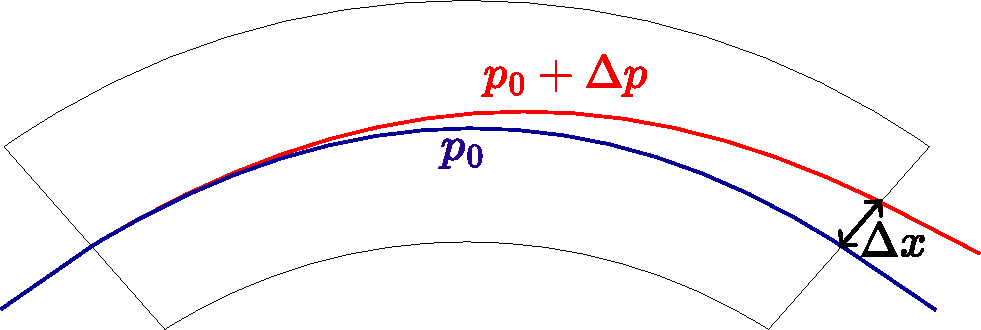
\includegraphics[width=0.6\textwidth]{images/dipole.pdf}
    \caption{Particles with a momentum offset will be deflected differently by dipoles. This offset
            in position can be described by the dispersion function.}
    \label{fig:coordinate_systems:dispersion}
\end{figure}

The particle is still subject to the other properties of the lattice, but with a different orbit,
described by Eq.~\eqref{fig:coordinate_systems:dispersion}.

\begin{equation}
    \begin{aligned}
    D_x(s) = \frac{\Delta x(s)}{\delta} \\
    D_y(s) = \frac{\Delta y(s)}{\delta} \\
    \end{aligned}
    \label{eq:coordinate_systems:dispersion}
\end{equation}



% ============================================
%               Beta Function
% ============================================
\subsection{\todo{$\beta$-function}}

As seen previously in~\ref{section:courant_snyder}, the $\beta$-function is related to the amplitude
of oscillations of the beam. Figure~\ref{fig:beam_optics:beta} shows how the $\beta$-function
oscillates along the ring due to quadrupoles focusing and defocusing properties.
The $\beta$-function is an important quantity found as a factor in several other observables that
will be described later in this thesis.


\begin{figure}[H]
    \centering
    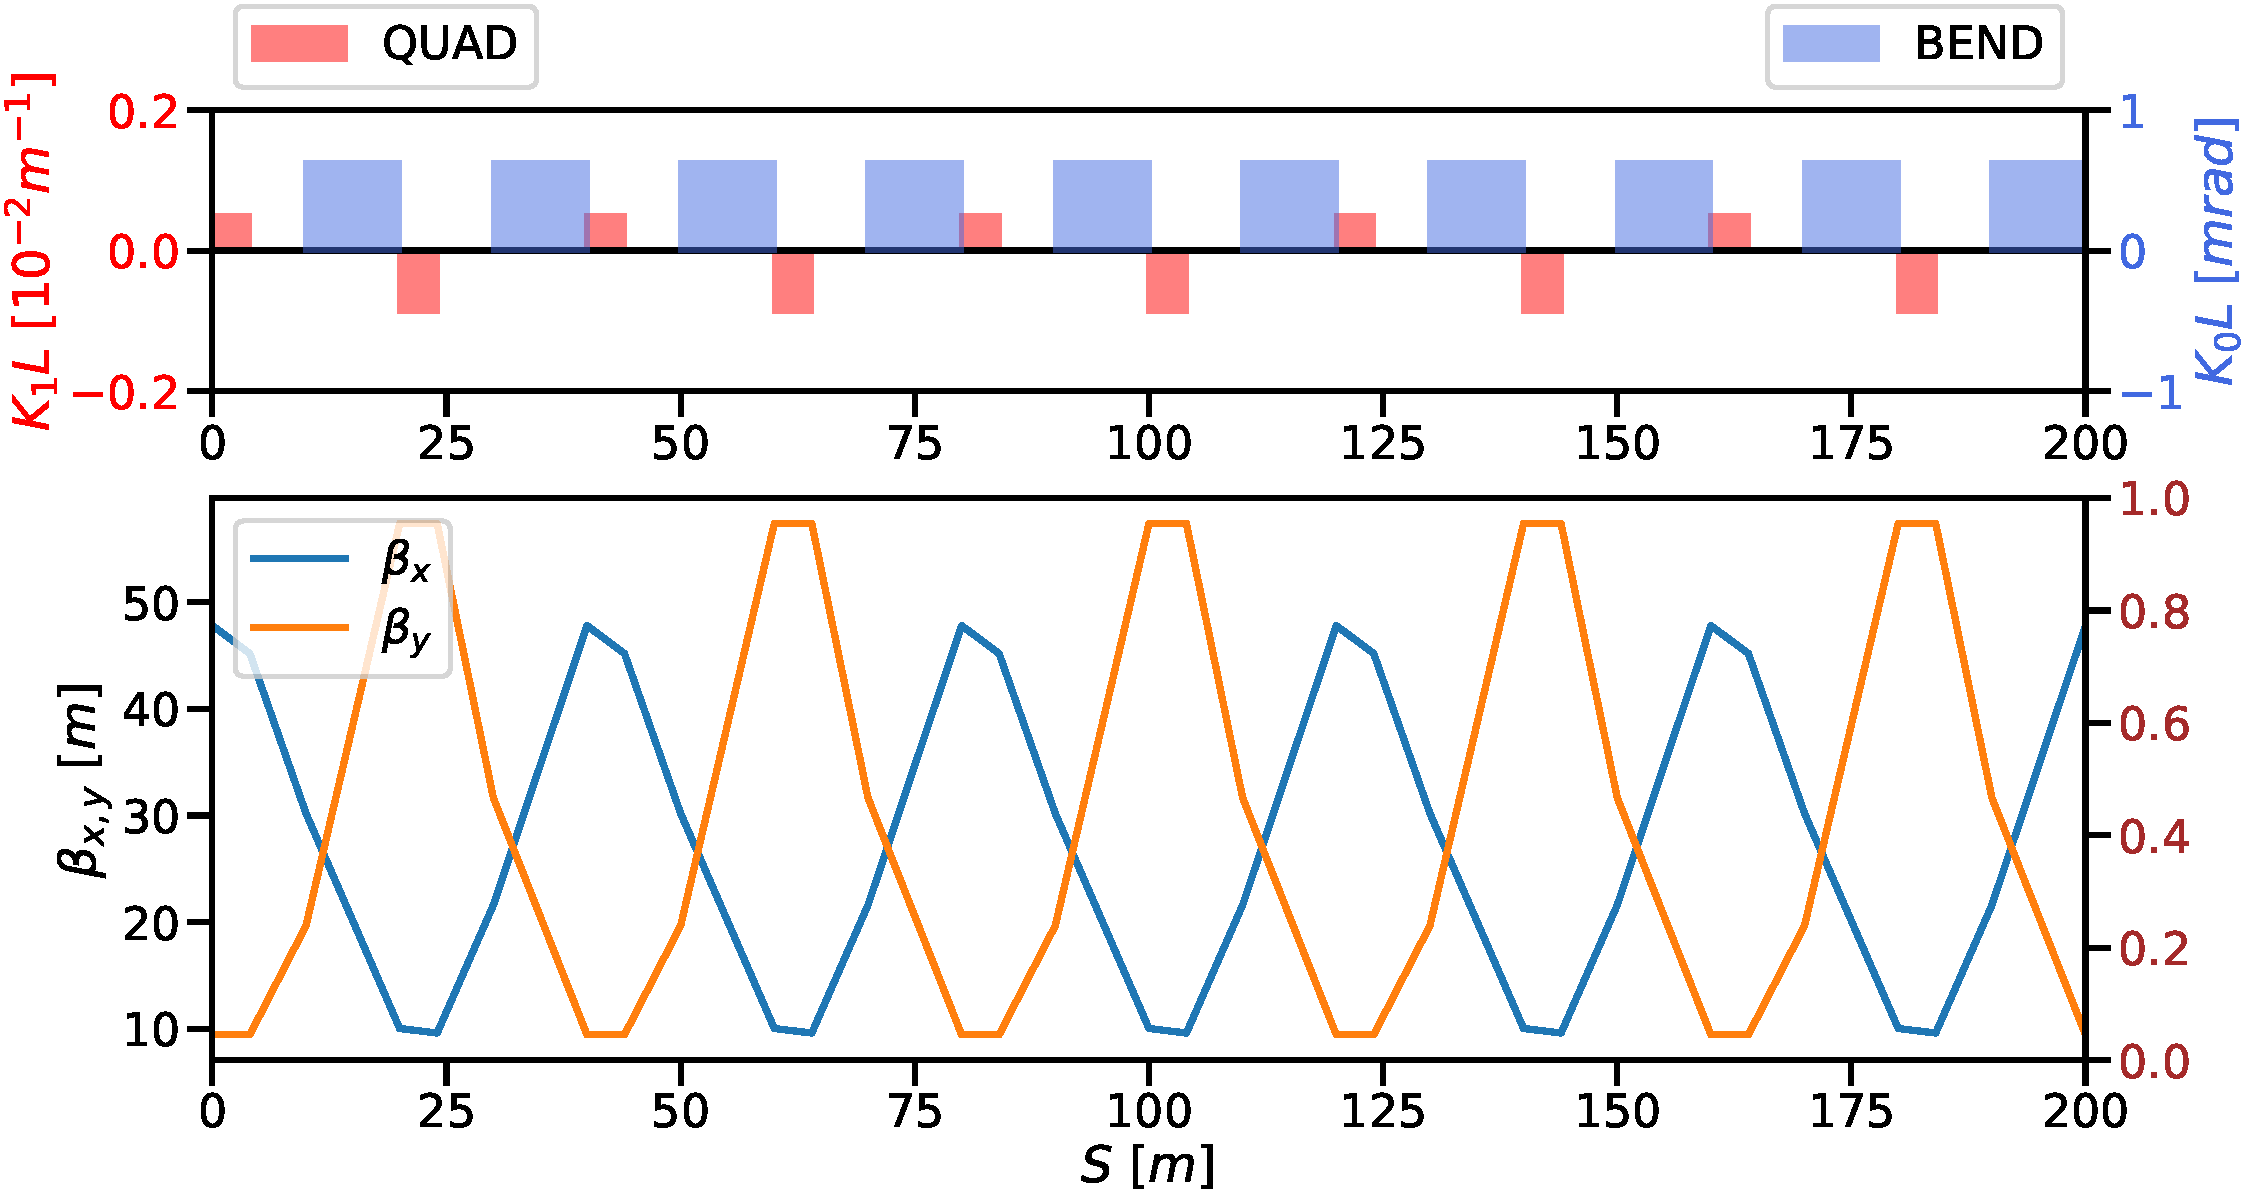
\includegraphics[width=0.9\textwidth]{images/beta_function.pdf}
    \caption{Evolution of the $\beta$-function along the lattice. Horizontal and vertical beatings
    are usually opposite given the focusing and defocusing properties of quadrupoles in each plane.}
    \label{fig:beam_optics:beta}
\end{figure}

A difference in $\beta$-function compared to the design leads to possible unstable and larger beams,
degrading its properties and making it harder to control. The relative difference in
$\beta$-function is called the beta-beating, expressed in percents: 

\begin{equation}
    \mathrm{beating \; [\%]}  = \frac{\beta_z(s) - \beta_z(s)_{model}}{\beta_z(s)_{model}}.
    \label{eq:beam_optics:beating}
\end{equation}


% ============================================
%                  Coupling
% ============================================
\subsection{\todo{Coupling}}


% ============================================
%         Momentum Compaction Factor
% ============================================
\subsection{\todo{Momentum Compaction Factor}}

